\genHeader
\newpage


\section*{A few words before you start}

This handbook has been engineered to be \emph{fun}.

If you work through it and, for some reason, do \emph{not} have a resounding \mbox{\enquote{I-Rule}} feeling afterwards, please send us an email and tell us how to improve it at \eMoflonContact.

\begin{figure}[htp]
\begin{center}
	
\includegraphics[height=0.45\textheight]{../introduction_images/i-rule}
	\caption{How you should feel when you're done}
	\label{i-rule}
\end{center}
\end{figure}
\break
 

To enjoy the experience, you should be fairly comfortable with Java or a comparable object-oriented language, and know how to perform basic tasks in Eclipse. 
Although we assume this, we give references to help bring you up to speed as necessary.
Last but not least, basic knowledge of common UML notation would be helpful.

Our goal is to give a \emph{hands-on} introduction to metamodelling and graph transformations using our tool \emph{eMoflon}.
The idea is to \emph{learn by doing} and all concepts are introduced while working on a concrete example.
The language and style used throughout is intentionally relaxed and non-academic.


\subsection*{So, what is eMoflon?}

eMoflon is a tool for building tools.
If you wish, a \enquote{meta} tool. 
This means that if you're interested in building \emph{domain-specific} tools for end users, then eMoflon could be pretty useful for you.


\subsection*{Why should I be interested?}

To build a tool, you typically need a way for users to communicate with it, \idest, you must establish a suitable \emph{language} for specifying input and output to and from the tool.
You also need a central data structure to represent the \enquote{state} of the tool.
This data structure or \emph{model} is usually manipulated and appropriately \emph{transformed} in some useful manner by the tool.
Many tools also \emph{generate} something useful from their internal models and keep them synchronized with other models in different tools.
To achieve these goals you can use \emph{metamodeling} to define your language (your \emph{meta}model), \emph{graph transformations} to transform your models.
All this and much more is supported by eMoflon.
Take a look at \Cref{fig:transformationModel} to see how all these tasks fit together.

\subsection*{What does this handbook cover?}

On the last page of this document, we've described each of the five parts that make up this handbook.
You can work through them sequentially and become an \emph{official}\footnote{Certificate not guaranteed} eMoflon master or, depending on your interests, decide what you'd like to read and what to skip.
We provide all the necessary materials (\idest, a cheat package) so you can jump right in without having to complete the previous parts. 
For those of you interested in further details and the mature formalism of graph transformations, we give relevant references throughout the handbook.

\begin{figure}[htbp]
	\centering
  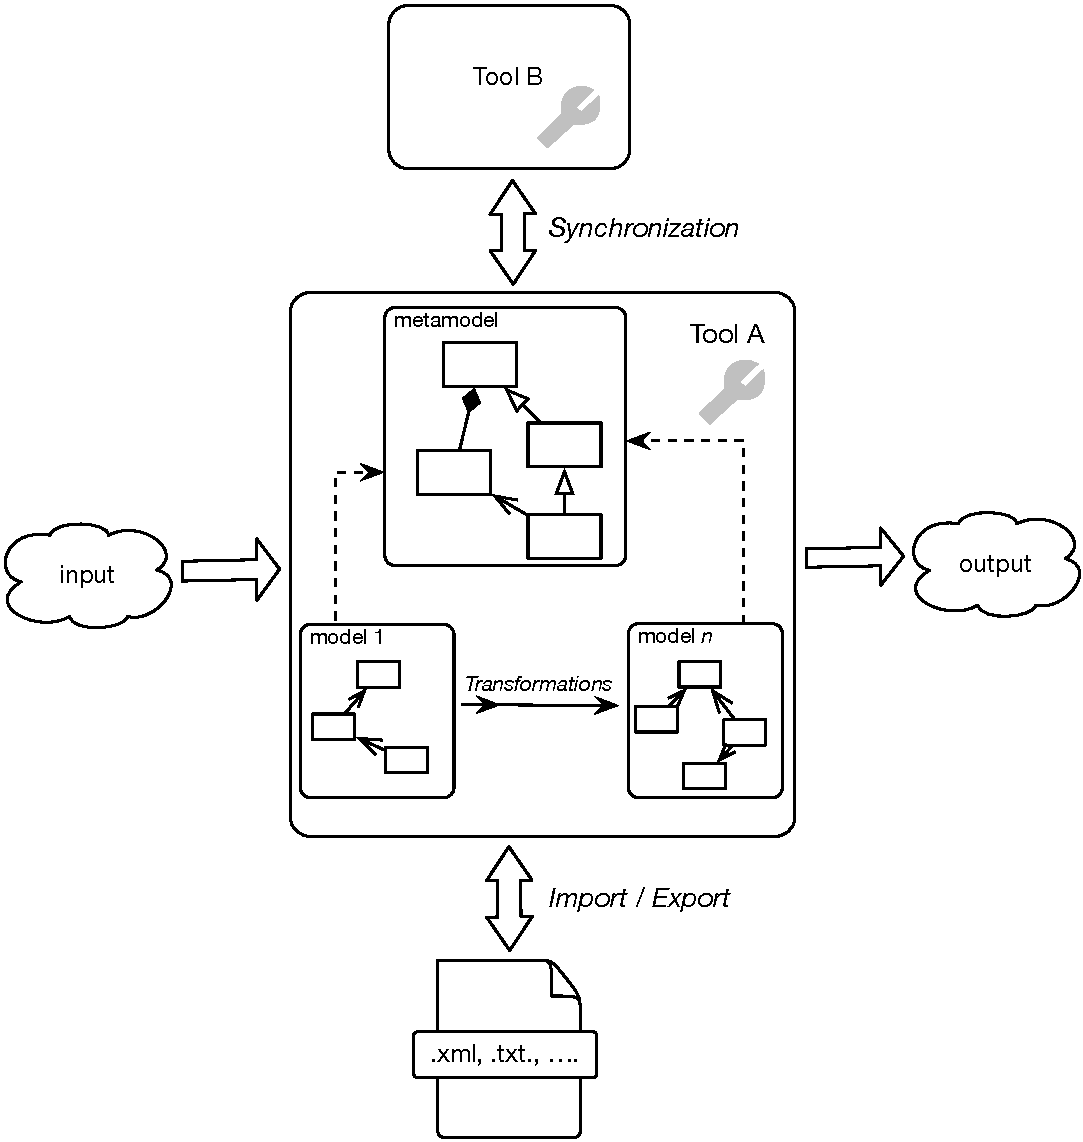
\includegraphics[width=0.9\textwidth]{eMoflonDiagram.pdf}
	\caption{Building a tool requires language specification (metamodeling), transformations, synchronization, and code generation}
	\label{fig:transformationModel}
\end{figure}
\begin{description}

\pagebreak

\item[\Cref{chap:installation}: Installation and set up] provides a very simple example and a few JUnit tests to test the installation and configuration of eMoflon.
We also explain the general workflow and the different workspaces involved.

This part can be considered \emph{mandatory} only if you are new to eMoflon, but we recommend working through it anyway.

\item[\Cref{chap:ecore}: Ecore] takes you step-by-step through a more realistic example that showcases many of the features we currently support.
Working through this part should serve as a basic introduction to model-driven engineering, and is especially recommended if you're new to metamodeling
(using Ecore and the Eclipse Modeling Framework (EMF)).


\item[\Cref{chap:sdm}: Story Driven Modelling (SDM)] introduces \emph{unidirectional} model transformation via programmed graph transformation using story diagrams (SDMs).


\item[\Cref{chap:Learning-Box-to-Dictionary-and-Back-Again}: Triple Graph Grammars (TGGs)] introduces \emph{bidirectional} model transformation with Triple Graph Grammars (TGGs).


\item[\Cref{chap:misc}: Miscellaneous] contains a collection of tips and tricks to keep
on hand while using eMoflon. This can be used as a reference to help avoid common mistakes and increase productivity. If you're in a hurry, this part can be skipped and consulted only on demand.

\end{description}

Well, that's it! Scroll down to \Cref{chap:installation}, grab a coffee, and enjoy the ride!
